For the derivation and the discussion of the relevant forces coming from the 
scattering of an axisymmetric incident acoustic field at the object surface, we 
will consider a viscous fluid and a rigid spherical particle. The particle is 
freely floating in the fluid and far away from any boundaries. We choose this 
combination of fluid and particle model for two reasons: 1) we discovered 
errors that we corrected in the publication solving this problem 
first~\cite{Doinikov1994Rigid}; 2) the viscous property of the fluid causes the 
occurrence of the so-called acoustic streaming (AS).

We will follow closely the derivations given by \cname{Doinikov1994Rigid} who 
solves this specific problem first \footnote{We will cite publications in this 
chapter only if they are different to \cname{Doinikov1994Rigid}. Per default, 
all information for this chapter if not stated otherwise is taken from there.}.

\section{Governing Equations}

Ultimately we want to compute the force acting on the particle. This force is 
called acoustic radiation force (ARF) and is defined as the time-averaged 
surface integral of the stress tensor over the time varying particle surface 
$S(t)$ (see \cref{fig:TA-deformed_circle})
\begin{equation}
  F^{\MR{rad}}_{i} \coloneqq
  \timeaverage{\int_{S(t)}\,\stress\,\normal(t)\,\dd{S(t)}}
  \label{eq:TA-def-rad}
\end{equation}
where $\normal(t)$ is the time dependent outward facing normal, repetitive 
indices imply Einstein summation notation, and the angle bracket define the 
time-average over one period $T_{\MR{ex}}$ of the fundamental excitation 
frequency $\fex=\nicefrac{1}{T_{\MR{ex}}}$ of the acoustic field
\begin{equation}
  \timeaverage{\Box(t)} = 
  \frac{1}{T_{\MR{ex}}}\,\int\limits_{0}^{T_{\MR{ex}}}\Box(t)\dd{t}.
  \label{eq:TA-time-average}
\end{equation}

\begin{figure}[tbp]
  \centering
  % \tikzsetnextfilename{deformed_circle}

\pgfmathsetmacro{\R}{2.25}     % COS
\begin{tikzpicture}
  \fill[colFluid,opacity=0.3] (-4.6,-2.6) rectangle (4.6, 2.6);
  \pgfmathsetseed{1} % choose a number which give a good shape to your circle
  \path[draw, fill=white,color=white] plot[domain=0:350,smooth cycle] 
  (\x:2+rnd*0.5);

  % axes
  \draw[ultra thin] (-2.5, 0) -- (2.5, 0);
  \draw[ultra thin] (0, -2.5) -- (0, 2.5);
  % undistorted sphere
  \draw[ultra thin, dashed] (0, 0) circle (\R);
  % distrorted sphere
  \pgfmathsetseed{1} % choose a number which give a good shape to your circle
  \path[draw, shading=ball, ball color=colParticle, fill opacity=0.3, thick, 
  name path=curve] plot[domain=0:350,smooth cycle] (\x:2+rnd*0.5);

  \draw[ultra thin, dashed, ->] (0:0) -- node[below, midway] {$R$} (190:\R);

  \draw[-] (140:\R) to[out=50, in=0] ++(-.4*\R,.25*\R) node[left] 
  {$\zeOrder{S}$};

  \path[very thick, name path=line] (0:0) -- (60:3.5);
  \draw [name intersections={of=curve and line, by=x}];
  \draw[-] (x) to[out=-35, in=180] ++(.6*\R,-.25*\R) node[right] {$S(t)$};

  \path[very thick, name path=line] (0:0) -- (10:3.5);
  \draw [name intersections={of=curve and line, by=x}];
  \draw[thick, |->] (x) to (13:3.5) node[right] {$\normal(t)$};
\end{tikzpicture}

  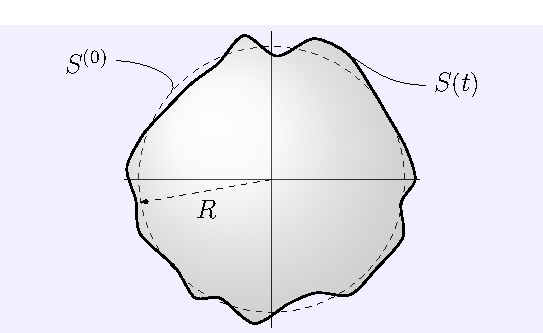
\includegraphics[]{/deformed_circle.pdf}
  \caption{Sketch of deformed time dependent particle surface $S(t)$, particle 
  surface at rest $\zeOrder{S}$, and time-varying surface normal $\normal(t)$.}
  \label{fig:TA-deformed_circle}
\end{figure}

For a viscous fluid the stress tensor is given as
\begin{equation}
  \stress = \muef\left[ \pdv{\vel_{i}}{x_{j}} + \pdv{\vel_{j}}{x_{i}} \right] + 
  \left[ \mu_{\MR{B}} - \frac{2}{3}\,\muef \right] \pdv{\vel_{k}}{x_{k}} 
  \,\delta_{ij} - \pre\,\delta_{ij}
  \label{eq:TA-stress}
\end{equation}
where $\muef$ is the fluid dynamic viscosity, $\mu_{\MR{B}}$ the fluid bulk 
viscosity, $\vel_{i}$ the $i$-th component of the fluid velocity, $\pre$ the 
pressure, and $\delta_{ij}$ the Kronecker delta.

For the stress tensor the fluid velocity $\vel_{i}$ and the acoustic pressure 
$\pre$ must be computed. These four unknowns (three as $\vel_{i}$ and one as 
$\pre$) are linked by the scalar equation for the mass conservation
\begin{equation}
  \pdv{\density}{t} + \pdv{x_{i}}(\density\,\vel_{i}) = 0
  \label{eq:TA-massconservation}
\end{equation}
where $\density$ is the density. This equation introduces the additional 
unknown density $\density$. With the assumption of a barotropic fluid
\begin{equation}
  \pre \coloneqq \pre\left( \density \right)
  \label{eq:TA-state}
\end{equation}
the acoustic pressure $\pre$ is defined solely by the density $\density$. The 
missing three equations are given by the Navier-Stokes equations for a viscous 
fluid
\begin{equation}
  \pdv{t}\left( \density\,\vel_{i} \right) = \pdv{x_{j}} \left( \stress - 
  \density\,\vel_{i}\,\vel_{j} \right).
    \label{eq:TA-navierconservative}
\end{equation}

% With the assumption, that the density $\density$ is constant in time and space 
% ($\pdv{\density}{t} = 0$, $\pdv{\density}{x_{i}} =0$)
% \cref{eq:TA-navierconservative} can be rearranged to
% \begin{equation}
  % \density\left( \pdv{\vel_{i}}{t} + \vel_{i}\pdv{\vel_{j}}{x_{j}}\right) = 
  % \pdv{\stress}{x_{j}}.
  % \label{eq:TA-navier}
% \end{equation}

This set of equations 
(\cref{eq:TA-massconservation,eq:TA-state,eq:TA-navierconservative}) describe 
the problem of a free floating rigid particle in a viscous fluid but are 
impossible to solve analytically without further simplification. Most common is 
the expansion of the unknowns into a converging 
% -- not guaranteed~\cite{Baasch2020} --
series of increasing order
\begin{subequations}
\begin{alignat}{4}
  \pre & = \zeOrder{\pre} & + \stOrder{\pre} & + \ndOrder{\pre} & + \ldots 
  \label{eq:TA-per-pre}\\
  \density & = \zeOrder{\density} & + \stOrder{\density} & + \ndOrder{\density} & + \ldots 
  \label{eq:TA-per-rho}\\
  \stress & = \zeOrder{\stress} & + \stOrder{\stress} & + \ndOrder{\stress} & + 
  \ldots \label{eq:TA-per-stress} \\
  \vel_{i} & =  & \phantom{+} \stOrder{\vel_{i}} & + \ndOrder{\vel_{i}} & + 
  \ldots \label{eq:TA-per-vel}.
\end{alignat}
\end{subequations}
This method of expanding the variables is called perturbation expansion. The 
superscript $\Box^{(i)}$ indicates the $i$-th order of the respective 
parameter. The zeroth order fields $\zeOrder{\Box}$ are defined to be constant 
in space and time. Additionally, we assume no constant flow of the fluid and, 
hence, the zeroth order of the velocity $\zeOrder{\vel_{i}} = 0$.

This series expansion is useful because it is known that the ARF occurs due to 
second order effects. With that the ARF is approximated \cref{eq:TA-def-rad} as
\begin{equation}
  F^{\MR{rad}}_{i} \approx
  \timeaverage{\int_{S(t)}\,\stOrder{\stress}\,\normal(t)\,\dd{S(t)}} +
  \int_{\zeOrder{S}}\,\timeaverage{\ndOrder{\stress}}\,
  \normal\,\dd{\zeOrder{S}}
  \label{eq:TA-def-approx-ARF}
\end{equation}
where $\zeOrder{S}$ is the particle surface at rest (see 
\cref{fig:TA-deformed_circle}).

It is possible to solve first for the first order fluid field, which is the 
acoustic field including scattering, and then use the first order solution to 
compute the second order fields, also known as AS. In the following two 
section, we will solve those two orders sequentially.

\section{First Order Solution\label{sec:TA-firstorder}}

By applying the perturbation expansion to \cref{eq:TA-massconservation} and by 
only collecting terms that are equal to the first order the mass conservation 
is
\begin{equation}
  \pdv{\stOrder{\density}}{t} + 
  \zeOrder{\density}\,\pdv{\stOrder{\vel_{i}}}{x_{i}} = 0.
  \label{eq:TA-st-massconservation}
\end{equation}

With the same procedure the general Navier Stockes equation 
(\cref{eq:TA-navierconservative}) is
\begin{equation}
  \zeOrder{\density} \pdv{\stOrder{\vel_{i}}}{t} = 
  \pdv{\stOrder{\stress}}{x_{j}}.
  \label{eq:TA-st-navier}
\end{equation}
with the first order stress tensor $\stOrder{\stress}$ being
\begin{equation}
  \stOrder{\stress} = \muef\left[ \pdv{\stOrder{\vel_{i}}}{x_{j}} + 
  \pdv{\stOrder{\vel_{j}}}{x_{i}} \right] + \left[ \mu_{\MR{B}} - 
  \frac{2}{3}\,\muef \right] \pdv{\stOrder{\vel_{k}}}{x_{k}} \,\delta_{ij} - 
  \stOrder{\pre}\,\delta_{ij}.
  \label{eq:TA-st-stress}
\end{equation}

The acoustic pressure of first order is
\begin{equation}
  \stOrder{\pre} = c^{2}\,\stOrder{\density}
  \label{eq:TA-st-pre}
\end{equation}
with $c$ being the speed of sound.

The first order velocity field $\stOrder{\vel_{i}}$ can be approximated as
\begin{equation}
  \stOrder{\vel}_{i} = \pdv{\stOrder{\phi}}{x_{i}} + 
  \epsilon_{kli}\,\pdv{\stOrder{\psi}_{l}}{x_{k}}
  \label{eq:TA-st-vel}
\end{equation}
where $\phi$ is the scalar velocity potential, $\psi_{i}$ the vector velocity 
potential, and $\epsilon_{kli}$ the Levi-Civita symbol to express the curl of 
the vector velocity potential in index notation. Furthermore, the scalar can be 
split up into the contributions from the incident velocity potential 
$\phi_{\MR{in}}$ and the scattered velocity potential $\phi_{\MR{sc}}$
\begin{equation}
  \stOrder{\phi} = \phi_{\MR{in}} + \phi_{\MR{sc}}.
  \label{eq:TA-scalar-potential}
\end{equation}

For the derivations we assume an axisymmetric incoming field and with the 
wavevector $\vb{k}$ pointing along the $\ez$ direction (see 
\cref{fig:TA-plane_wave}). Additionally, we use spherical coordinates $r, 
\theta$, and $\varphi$ with the origin at the center of the particle in its 
equilibrium configuration (see \cref{fig:TA-coordinate}).

\begin{figure}[tbp]
  \centering
  % \tikzsetnextfilename{plane_wave}
%----------------------
%Plot display orientation
\pgfmathsetmacro{\thetaC}{80}
\pgfmathsetmacro{\phiC}{100}
\tdplotsetmaincoords{\thetaC}{\phiC}
%----------------------
%Parameters 
\pgfmathsetmacro{\R}{4}     % COS
\pgfmathsetmacro{\k}{2.7}   % distance k vector
\pgfmathsetmacro{\rvec}{2}  % Particle's radius
\pgfmathsetmacro{\l}{4}   % width of planar wave
\pgfmathsetmacro{\endl}{7}  % Azimuthal dashed line

\begin{tikzpicture}[tdplot_main_coords]
\coordinate (O) at (0,0,0);
\coordinate (X) at (\R,0,0);
\coordinate (Y) at (0,0,\R);
\coordinate (Z) at (0,\R,0);
\tdplotsetcoord{P}{2*\R}{-90}{0}

%----------------------
% Particle
\shadedraw[tdplot_screen_coords,particle, opacity=.4](O) circle (\rvec);
% Edges for labels
\draw[-](0,.3*\R,.2*\R) to[out=40, in=180] ++(0,.4*\R,.45*\R)
    node[right] {Particle};
%-----------------------
% Radial
    \draw[thick,dashed] (O) -- (P);
    %\tdplotdrawarc[->]{(P)}{0.7}{0}{90}{anchor=north}{$\theta$}
\pic [draw, ->, "$\theta$", angle eccentricity=1.2,angle radius=1cm] {angle = Z--O--P};
%-----------------------
% Equator
\draw[dashed] (\rvec,0,0) arc (0:360:\rvec);
% Draw the arc which center is (O) from \phiC to \phiC-180 deg
\draw[thick] ([shift=(\phiC:\rvec)]O) arc (\phiC:\phiC-180:\rvec);
%-----------------------
% Cartesian COS
\begin{scope}[->,thick]
    \draw (O) -- (X)
        node[anchor=north east]{$\ey$};
    \draw (O) -- (Y)
        node[anchor=north west]{$\ex$};
  \draw (O) -- (Z)
    node[anchor=south east]{$\ez$};
\end{scope}
%----------------------
%----------------------
% Axis of symmetry
\draw[dashed] ($(O)+(0,\endl-1.5,0)$) -- (0,-\endl+1,0);
% Edges for labels
\draw[-] ($(O)+(0,\endl-2,0)$) to[out=120, in=-90] ++($(O)+(0,\endl-8,.25*\R)$)
    node[above]{Axis of symmetry};
%----------------------
% Incoming wave vector
\coordinate (P) at (0,-\k,0);
\draw[->,thick,color=red] (0,-1.5*\k,0) -- (P) 
node[above,pos=.6]{$\vb{k}=k\vb{e}_{\MR{k}}$};
 %----------------------
% Incoming wave fronts
\foreach \z in {-7,-6,-5}
\draw [red, fill=red!20, opacity=.4] plot (\l,\z,1) -- (-\l,\z,1) --(-\l,\z,-1) -- (\l,\z,-1) -- cycle;
\end{tikzpicture}



  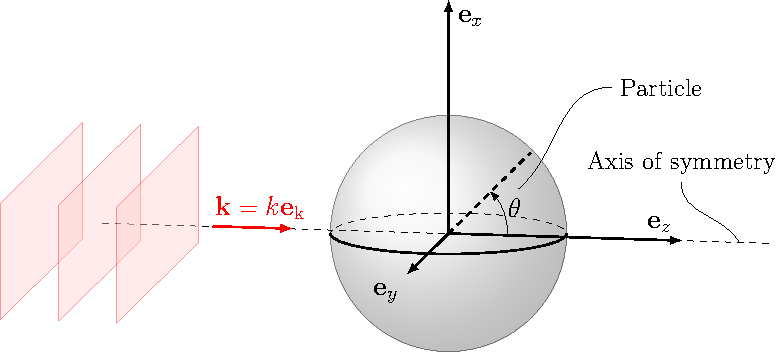
\includegraphics[]{/plane_wave.pdf}
  \caption{Plane acoustic wave incident on spherical particle. Wavevector 
  direction $\vb{e}_{\MR{k}}$ aligned with $\ez$.}
  \label{fig:TA-plane_wave}
\end{figure}

For the general case, the scalar incident velocity potential can be represented 
as
\begin{equation}
  \phi_{\MR{in}} = \exp\left( -\iu\omega t \right) \sum\limits_{n=0}^{\infty} 
  A_{n}\,\bessel{n}{kr}\,\legendre{n}{\cos\,\theta}
  \label{eq:TA-incident-field}
\end{equation}
where $\omega=2\pi\,\fex$ is the angular frequency of the incoming acoustic 
wave, $t$ the time, $A_{n}$ the amplitude of the incoming wave, 
$\bessel{n}{\Box}$ the $n$-th order spherical Bessel function of first kind, 
$\legendre{n}{\Box}$ the Legendre polynomial of order $n$, and $k$ the 
wavenumber
\begin{equation}
  k = 
  \frac{\omega}{c}\,\frac{1}{\sqrt{1-\frac{\iu\,\omega}{\zeOrder{\density}\,c^{2}} 
  \left( \mu_{\MR{B}} + \frac{4}{3}\,\muef \right)}}.
  \label{eq:TA-wavenumber}
\end{equation}

The amplitudes $A_{n}$ of \cref{eq:TA-incident-field} are known by the type of 
incident wave (traveling, standing, spherical). $\phi_{\MR{sc}}$ and 
$\stOrder{\psi_{i}}$ can be separated into two independent differential 
equations. For $\phi_{\MR{sc}}$ we take first \cref{eq:TA-scalar-potential} 
and plug it into the mass conservation \cref{eq:TA-st-massconservation}. With 
the property that the divergence of the curl is equal to zero
\begin{equation}
  \pdv{x_{i}}\left[\epsilon_{kli}\pdv{\Box_{l}}{x_{k}}\right] = 0
\end{equation}
and the definition of the first order pressure \cref{eq:TA-st-pre} one can 
eliminate $\psi_{i}$ completely
\begin{equation}
  \pdv{\stOrder{\pre}}{t} = 
  \zeOrder{\density}\,c^{2}\,\pdv[2]{\stOrder{\phi}}{x_{i}}.
  \label{eq:TA-st-tmp-step}
\end{equation}
The next step is to take \cref{eq:TA-st-tmp-step} and plug it into the partial 
time derivative ($\pdv{\Box}{t}$) of \cref{eq:TA-st-navier}. This results in a 
wave equation which can be further simplified because we assume time harmonic 
acoustics fields ($\vel_{i}\propto\exp -\iu\omega t$) that have the property 
$\pdv{\vel_{i}}{t}\propto -\iu\omega$ and
$\pdv[2]{\vel_{i}}{t}\propto \omega^{2}$
\begin{equation}
  \label{eq:TA-st-nd-tmp-step}
\begin{split}
  \zeOrder{\density}\,\pdv[2]{\stOrder{\vel_{i}}}{t} = & 
  \zeOrder{\density}\,c^{2}\pdv{x_{i}}\left( \pdv[2]{\stOrder{\phi}}{x_{j}} 
  \right) \\
  + & \mu\,\pdv[2]{x_{i}}\left( \pdv{\stOrder{\vel_{k}}}{t} \right) \\
    + & \left(\mu_{\MR{B}} + \frac{\mu}{3}\right)\pdv{t}
    \left( \pdv{x_{i}}\left( \pdv[2]{\stOrder{\phi}}{x_{j}} \right) \right).
\end{split}
\end{equation}

The last step is to take the divergence of \cref{eq:TA-st-nd-tmp-step} to 
eliminate $\stOrder{\psi_{i}}$. Finally, the equation for $\stOrder{\phi}$ is 
given as a Helmholtz equation
\begin{equation}
  \pdv[2]{\stOrder{\phi}}{x_{i}} + k^{2}\,\stOrder{\phi} = 0.
  \label{eq:TA-st-phi}
\end{equation}

\begin{figure}[tbp]
  \centering
  % \tikzsetnextfilename{coordinate}

\begin{tikzpicture}[line cap=round, line join=round, >=Triangle, scale=1.5]

\clip(-2.1,-2.1) rectangle (2.38,2.58);
\filldraw[blue!20,opacity=.3] (-2.1,-2.1) rectangle (2.38,2.58);
\filldraw[white] (0,0) circle (2cm);

\draw[ball color=gray!20!white, fill opacity=0.6] (0,0) circle (2cm);

\draw [rotate around={0.:(0.,0.)},dash pattern=on 3pt off 3pt] (0,0) ellipse 
(2cm and 0.9cm);

\draw (0,0) -- (0.70,1.07) node[right, pos=0.4] {$r$};


\draw[-latex,line width=0.7pt]   (0,0) -- +(0,2) node[above] {$\ez$};
\draw[-latex,line width=0.7pt]   (0,0) -- +(-0.83,-0.81) node [left, 
yshift=-1.8mm] {$\ex$};
\draw[-latex,line width=0.7pt]  (0,0) -- +(2,0) node [right] {$\ey$};


\draw [-Latex, <-, >=stealth', shift={(0,0)}, black, fill opacity=1] (56.7:0.4) 
arc (56.7:90.:0.4) node[above, pos=0.3] {$\theta$};

\begin{scope}[rotate around x=10, y=10, xshift=1, yshift=-4.6]
    \draw [-Latex, ->, >=stealth', shift={(0,0)}, black, fill opacity=1] 
    (-135.7:0.4) arc (-135.7:-33.2:0.4) node[below,pos=0.4] {$\varphi$};
\end{scope}

\draw [dotted] (0.7,1)-- (0.7,-0.46);
\draw [dotted] (0,0)-- (0.7,-0.46);
\draw [fill] (0,0) circle (1.5pt);
\draw [fill] (0.7,1.07) circle (0.5pt);
\end{tikzpicture}

  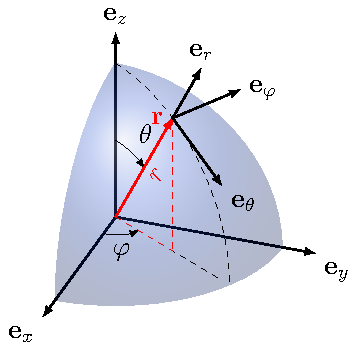
\includegraphics[]{/coordinate.pdf}
  \caption{Sketch of Cartesian and spherical coordinate system}
  \label{fig:TA-coordinate}
\end{figure}

Instead of taking the divergence of \cref{eq:TA-st-nd-tmp-step} but taking the 
curl one gets a Helmholtz equation for $\stOrder{\psi_{i}}$
\begin{equation}
  \pdv[2]{\stOrder{\psi_{j}}}{x_{i}} + k_{\MR{v}}^{2}\,\stOrder{\psi_{i}} = 0
  \label{eq:TA-st-psi}
\end{equation}
by using $\epsilon_{kli}\,\pdv{x_{k}}\left( \pdv{\Box}{x_{l}} \right) = 0$ 
(curl of the gradient of a scalar). In \cref{eq:TA-st-psi} $k_{\MR{v}}$ is 
called the viscous wavenumber and is defined as
\begin{equation}
  k_{\MR{v}} = \frac{1 + \iu}{\delta} = \left( 1 + \iu \right)\, 
  \sqrt{\frac{\omega\,\zeOrder{\density}}{2\rhof}}
  \label{eq:TA-st-visc-wavenumber}
\end{equation}
where $\delta$ is also known as the viscous boundary layer (VBL) thickness.

With the requirement that the solutions to \cref{eq:TA-st-phi,eq:TA-st-psi} 
satisfy Sommerfeld's radiation condition and using multipole expansion one 
finds
\begin{equation}
  \phi_{\MR{sc}} = \exp\left( -\iu\omega t \right)\,
  \sum\limits^{\infty}_{n=0} 
  \alpha_{n}\,A_{n}\,\hankel{n}{k\,r}\,\legendre{n}{\cos\theta}
  \label{eq:TA-st-sol-phi}
\end{equation}
and
\begin{equation}
  \vb*{\psi}^{(1)} = \exp\left( -\iu\omega t \right)\,\vb{e}_{\varphi}\,
  \sum\limits^{\infty}_{n=1} 
  \beta_{n}\,A_{n}\,\hankel{n}{k_{\MR{v}}\,r}\,P^{1}_{n}(\cos\theta)
  \label{eq:TA-st-sol-psi}
\end{equation}
where $\alpha_{n}$ and $\beta_{n}$ are constants defined by the boundary 
conditions, $\vb{e}_{\varphi}$ the unit vector of the spherical coordinate 
system (see \cref{fig:TA-coordinate}), $\hankel{n}{\Box}$ the spherical Hankel 
functions of the first kind, and $P^{1}_{n}\left( \Box \right)$ the associated 
Legendre polynomial. The sum of \cref{eq:TA-st-sol-psi} starts with $n=1$ 
because $\beta_{0}=0$.

The boundary condition for the combination of a rigid spherical particle and a 
viscous fluid is that the velocity of the particle $\vel_{\MR{p}}$ at the 
surface must match the fluid velocity there
\begin{equation}
  \vel_{i,\MR{fluid}} = \vel_{i,\MR{p}}\quad\text{at}\quad r = R.
  \label{eq:TA-st-BC}
\end{equation}

Using Newton's second law, the first order stress tensor, and the equilibrium 
particle surface $\zeOrder{S}$ as integration boundary such that the formula is 
accurate up to first order, one finds
\begin{equation}
  \underbrace{\frac{4}{3}\,\pi\,R^{3}\,\density_{\MR{p}}}_{m}
  \underbrace{\dv{\stOrder{\vel_{i,\MR{p}}}}{t}}_{a} = 
  \int\limits_{\zeOrder{S}}\stOrder{\stress}\normal\dd{\zeOrder{S}}
  \label{eq:TA-st-newton}
\end{equation}
where $\density_{\MR{p}}$ is the particle density, one finds the particle 
velocity along the direction of the wave vector $\vb{e}_{k}$ as
\begin{equation}
  \stOrder{\vel_{\MR{p}}} = \frac{\zeOrder{\density}A_{1}k}{x}\,
  \left[
    \bessel{1}{x} + \alpha_{1}\hankel{1}{x} + 2\beta_{1}\hankel{1}{\xv}
  \right]
  \,\exp\left( -\iu\omega t \right)
  \label{eq:TA-st-particle-vel}
\end{equation}
with $x=kR$ and $\xv=k_{\MR{v}}R$.

In order to calculate the unknown constants $\alpha_{n}$ and $\beta_{n}$ one 
needs to enforce the boundary condition of \cref{eq:TA-st-BC} for every $n$ 
separately. Besides for $n=1$, $\vel_{\MR{p}}$ is always zero because the 
multipole expansion for a rigid particle has only a dipole contribution; for 
$n=1$, $\stOrder{\vel_{\MR{p}}}$ is given by \cref{eq:TA-st-particle-vel}.

For $n=0$ and $n=1$ the constants $\alpha_{0}, \alpha_{1}, \beta_{0},$ and 
$\beta_{1}$ are
\begin{subequations}
\begin{align}
  \alpha_{0} & = -\frac{\bessel{1}{x}}{\hankel{1}{x}} \\
  \beta_{0} & = 0 \\
  \alpha_{1} & = - \frac{1}{\chi_{4}} \left[ \chi_{1}\,\chi_{3} + 
  2(1-\trho^{2})\bessel{1}{x}\hankel{1}{\xv} \right]
    \label{eq:TA-alpha-one}\\
    \beta_{1} &= - \frac{1-\trho}{\chi_{4}} \left[ \chi_{1}\,\hankel{1}{x} - 
    \chi_{2}\,\bessel{1}{x} \right]
    \label{eq:TA-beta-one}
\end{align}
\end{subequations}
where $\trho = \sfrac{\rhof}{\density_{\MR{p}}}$ and
\begin{subequations}
\begin{align}
\chi_{1} & = \trho\,\bessel{1}{x} - \trho\,\dbessel{1}{x}
\label{eq:TA-chi-one} \\
\chi_{2} & = \trho\,\hankel{1}{x} - \trho\,\dhankel{1}{x}
\label{eq:TA-chi-two} \\
\chi_{3} & = \left( 1 + 2 \trho\right)\hankel{1}{\xv} + 
\xv\,\dhankel{1}{x}
\label{eq:TA-chi-three} \\
\chi_{4} & = \chi_{2}\,\chi_{3} + 2\left( 1 - \trho^{2} \right) 
\hankel{1}{x}\,\hankel{1}{\xv}
\label{eq:TA-chi-four}
\end{align}
\end{subequations}
where the prime $\Box^{\prime}$ indicates the differentiation, e.g. 
$\dbessel{n}{\xv}=\dv{\bessel{n}{\xv}}{\xv}$.

For $n > 1$, one finds the coefficients $\alpha_{n}$ and $\beta_{n}$ to be
\begin{subequations}
\begin{align}
  \alpha_{n} & =
  - \frac{1}{\xi_{n}} \left[
    n(n+1)\bessel{n}{x}\hankel{n}{\xv} - x \gamma_{n}\dbessel{n}{x}
  \right]
  \label{eq:TA-alpha-n}\\
    \beta_{n} &= - \frac{1}{\xi_{n}} \left[
      x\dbessel{n}{x}\hankel{n}{x} - x\bessel{n}{x}\dhankel{n}{x}
    \right]
    \label{eq:TA-beta-n}
\end{align}
\end{subequations}
with
\begin{subequations}
\begin{align}
  \gamma_{n} & =
  \hankel{n}{\xv}+\xv\dhankel{n}{\xv}
  \label{eq:TA-gamma-n}\\
  \xi_{n} &= x\dhankel{n}{x}\gamma_{n} - n(n+1)\hankel{n}{x}\hankel{n}{\xv}.
    \label{eq:TA-xi-n}
\end{align}
\end{subequations}

\begin{table}
  \centering
  \begin{tabular}{lccr}
    \toprule
    \toprule
    {\bfseries Parameter} & {\bfseries Symbol} & {\bfseries Value} & {\bfseries 
    Unit}\\
    \midrule
    \textbf{Fluid} & & \\
    Density & $\rhof$ & 1000 & \si{\kg\per\cubic\meter} \\
    Speed of sound & $\cfl$ & 1500 & \si{\m\per\s} \\
    Dynamic viscosity (\SI{25}{\degreeCelsius}) & $\muef$ & 0.89 & 
    \si{\milli\pascal\second} \\
    Bulk viscosity (\SI{25}{\degreeCelsius}) & $\mu_{\MR{B}}$ & 2.47 & 
    \si{\milli\pascal\second} \\
    \midrule
    \textbf{Particle} & & \\
    Density & $\rhop$ & 1850 & \si{\kg\per\cubic\meter} \\
    Radius & $\R$& 1.03 & \si{\um}\\
    \midrule
    \textbf{Acoustic Field} & & \\
    Wavetype &  & travelling & - \\
    Pressure & $p_{\MR{a}}$ & 100.0 & \si{\kilo\pascal} \\
    Frequency & $\fex$ & 1.0 & \si{\MHz} \\
    \bottomrule
    \bottomrule
  \end{tabular}
  \caption{Symbols and physical properties of the fluid, the particle, and the 
  incident acoustic wave.}\label{tab:TA-parameters}
\end{table}

Note here, that 
\cref{eq:TA-alpha-one,eq:TA-beta-one,eq:TA-chi-three,eq:TA-chi-four,eq:TA-beta-n} 
are different from the equations in \cname{Doinikov1994Rigid} (Equations 
(3.14), (3.15), (3.18), (3.19), and (3.21), respectively). We discovered these 
typos in the original publication and discussed it more extensively in 
\cname{Fankhauser2022} with agreement of the author himself.

\begin{figure}
  \centering
  \begin{subfigure}[b]{\textwidth}
    \centering
    \caption{Modes up to $n=5$}
    % \tikzsetnextfilename{SC_all}

\renewcommand{\tikzHelper}{\relPath/10_Figures/TikZ/scattering_data}

\begin{tikzpicture}
\begin{groupplot}[
  group style={
    vertical sep=6mm,
    horizontal sep=3mm,
    group size= 2 by 3,
  },
  title style={yshift=-2.5mm,},
  xmin=-5,
  xmax=5,
  ymin=0,
  ymax=5,
  point meta max=75,
  point meta min=4,
  view={0}{90},
  % colorbar,
  colormap = {whiteblack}{color(0cm)  = (black);color(1cm) = (white)},
  % colormap/bluered,                     % Colormap preset
  height=4cm,
  width=75mm,
  ]

  %%%%%%%%%%%%%%%%
  \nextgroupplot[
    title={$\omega t =0\,\pi$},
    ylabel={$\sfrac{x}{R}$},
    xticklabels={,,},
]
    \addplot3[
        contour filled={number=25,labels={false}},
        mesh/rows=110,
        mesh/check=false
    ] table[x=z, y=x, z=c] {\tikzHelper/phase_0.dat};

    \coordinate (top) at (rel axis cs:0,1);
  %%%%%%%%%%%%%%%%
  \nextgroupplot[
    title={$\omega t =0.2\,\pi$},
    xticklabels={,,},
    yticklabels={,,},
]
    \addplot3[
        contour filled={number=25,labels={false}},
        mesh/rows=110,
        mesh/check=false
    ] table[x=z, y=x, z=c] {\tikzHelper/phase_1.dat};

  %%%%%%%%%%%%%%%%
  \nextgroupplot[
    title={$\omega t =0.4\,\pi$},
    ylabel={$\sfrac{x}{R}$},
    xticklabels={,,},
]
    \addplot3[
        contour filled={number=25,labels={false}},
        mesh/rows=110,
        mesh/check=false
    ] table[x=z, y=x, z=c] {\tikzHelper/phase_2.dat};

  %%%%%%%%%%%%%%%%
  \nextgroupplot[
    title={$\omega t =0.6\,\pi$},
    xticklabels={,,},
    yticklabels={,,},
]
    \addplot3[
        contour filled={number=25,labels={false}},
        mesh/rows=110,
        mesh/check=false
    ] table[x=z, y=x, z=c] {\tikzHelper/phase_3.dat};

  %%%%%%%%%%%%%%%%
  \nextgroupplot[
    title={$\omega t =0.8\,\pi$},
    ylabel={$\sfrac{x}{R}$},
    xlabel={$\sfrac{z}{R}$},
]
    \addplot3[
        contour filled={number=25,labels={false}},
        mesh/rows=110,
        mesh/check=false
    ] table[x=z, y=x, z=c] {\tikzHelper/phase_4.dat};

  %%%%%%%%%%%%%%%%
  \nextgroupplot[
    title={$\omega t =1.0\,\pi$},
    yticklabels={,,},
    xlabel={$\sfrac{z}{R}$},
]
    \addplot3[
        contour filled={number=25,labels={false}},
        mesh/rows=110,
        mesh/check=false
    ] table[x=z, y=x, z=c] {\tikzHelper/phase_5.dat};

  \coordinate (bot) at (rel axis cs:1,0);

\end{groupplot}
  \path (top-|current bounding box.east)--
                    coordinate(legendposright)
                    (bot-|current bounding box.east);


\begin{axis}[%
  hide axis,
  scale only axis,
  %height=0.975\linewidth,
  %width=0.01\linewidth,
  at={(legendposright.east)},
  anchor=east,
  xshift=60mm,
  point meta min=4.0,
  point meta max=75.0,
  % colormap/bluered,                     % Colormap preset
  colormap = {whiteblack}{color(0cm)  = (black);color(1cm) = (white)},
  colorbar right,                  % Active colorbar
  colorbar sampled,                     % Steps in colorbar
  colorbar style={
    separate axis lines,
    samples=256,                        % Number of steps
    ylabel={Acoustic Velocity $\abs{\vb{v}}$ [\si{\mm\per\second}]},
  },
  every colorbar/.append style={
    height=\pgfkeysvalueof{/pgfplots/parent axis height}%+
               %\pgfkeysvalueof{/pgfplots/group/vertical sep}
  }
]
  \addplot [draw=none] coordinates {(0,0)};
\end{axis}

\end{tikzpicture}

    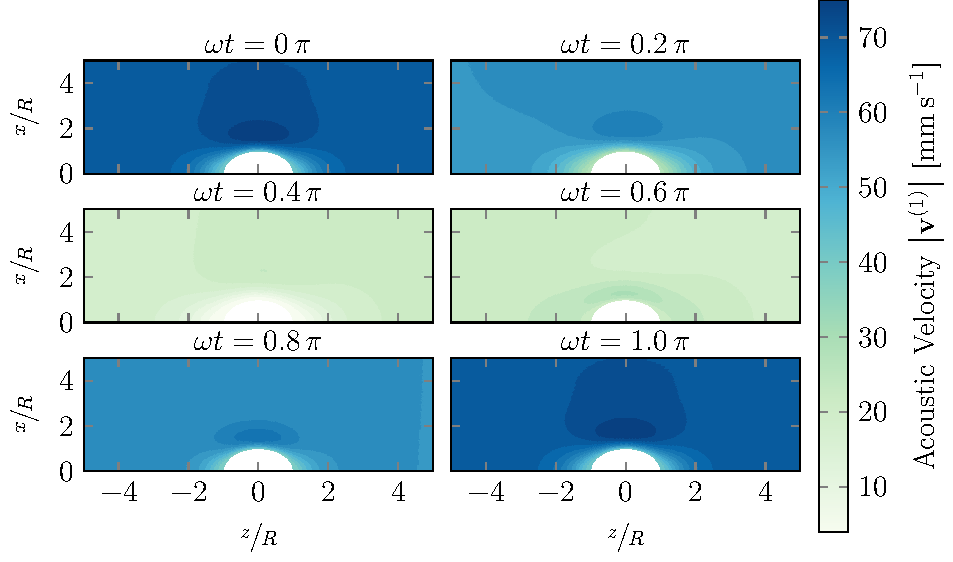
\includegraphics[]{/SC_all.pdf}
    \label{fig:TA-SC_all}
  \end{subfigure}\\%
  \begin{subfigure}[b]{\textwidth}
    \centering
    \caption{Single mode $n=1$}
    % \tikzsetnextfilename{SC_mode1}

\renewcommand{\tikzHelper}{\relPath/10_Figures/TikZ/scattering_data}

\begin{tikzpicture}
\begin{groupplot}[
  group style={
    vertical sep=6mm,
    horizontal sep=3mm,
    group size= 2 by 3,
  },
  title style={yshift=-2.5mm,},
  xmin=-5,
  xmax=5,
  ymin=0,
  ymax=5,
  point meta max=75,
  point meta min=4,
  view={0}{90},
  % colorbar,
  colormap = {whiteblack}{color(0cm)  = (black);color(1cm) = (white)},
  % colormap/bluered,                     % Colormap preset
  height=4cm,
  width=75mm,
  ]

  %%%%%%%%%%%%%%%%
  \nextgroupplot[
    title={$\omega t =0\,\pi$},
    ylabel={$\sfrac{x}{R}$},
    xticklabels={,,},
]
    \addplot3[
        contour filled={number=25,labels={false}},
        mesh/rows=110,
        mesh/check=false
    ] table[x=z, y=x, z=c] {\tikzHelper/phase_0_mode_1.dat};

    \coordinate (top) at (rel axis cs:0,1);
  %%%%%%%%%%%%%%%%
  \nextgroupplot[
    title={$\omega t =0.2\,\pi$},
    xticklabels={,,},
    yticklabels={,,},
]
    \addplot3[
        contour filled={number=25,labels={false}},
        mesh/rows=110,
        mesh/check=false
    ] table[x=z, y=x, z=c] {\tikzHelper/phase_1_mode_1.dat};

  %%%%%%%%%%%%%%%%
  \nextgroupplot[
    title={$\omega t =0.4\,\pi$},
    ylabel={$\sfrac{x}{R}$},
    xticklabels={,,},
]
    \addplot3[
        contour filled={number=25,labels={false}},
        mesh/rows=110,
        mesh/check=false
    ] table[x=z, y=x, z=c] {\tikzHelper/phase_2_mode_1.dat};

  %%%%%%%%%%%%%%%%
  \nextgroupplot[
    title={$\omega t =0.6\,\pi$},
    xticklabels={,,},
    yticklabels={,,},
]
    \addplot3[
        contour filled={number=25,labels={false}},
        mesh/rows=110,
        mesh/check=false
    ] table[x=z, y=x, z=c] {\tikzHelper/phase_3_mode_1.dat};

  %%%%%%%%%%%%%%%%
  \nextgroupplot[
    title={$\omega t =0.8\,\pi$},
    ylabel={$\sfrac{x}{R}$},
    xlabel={$\sfrac{z}{R}$},
]
    \addplot3[
        contour filled={number=25,labels={false}},
        mesh/rows=110,
        mesh/check=false
    ] table[x=z, y=x, z=c] {\tikzHelper/phase_4_mode_1.dat};

  %%%%%%%%%%%%%%%%
  \nextgroupplot[
    title={$\omega t =1.0\,\pi$},
    yticklabels={,,},
    xlabel={$\sfrac{z}{R}$},
]
    \addplot3[
        contour filled={number=25,labels={false}},
        mesh/rows=110,
        mesh/check=false
    ] table[x=z, y=x, z=c] {\tikzHelper/phase_5_mode_1.dat};

  \coordinate (bot) at (rel axis cs:1,0);

\end{groupplot}
  \path (top-|current bounding box.east)--
                    coordinate(legendposright)
                    (bot-|current bounding box.east);


\begin{axis}[%
  hide axis,
  scale only axis,
  %height=0.975\linewidth,
  %width=0.01\linewidth,
  at={(legendposright.east)},
  anchor=east,
  xshift=60mm,
  point meta min=4.0,
  point meta max=75.0,
  % colormap/bluered,                     % Colormap preset
  colormap = {whiteblack}{color(0cm)  = (black);color(1cm) = (white)},
  colorbar right,                  % Active colorbar
  colorbar sampled,                     % Steps in colorbar
  colorbar style={
    separate axis lines,
    samples=256,                        % Number of steps
    ylabel={Acoustic Velocity $\abs{\stOrder{\vb{v}}}$ [\si{\mm\per\second}]},
  },
  every colorbar/.append style={
    height=\pgfkeysvalueof{/pgfplots/parent axis height}%+
               %\pgfkeysvalueof{/pgfplots/group/vertical sep}
  }
]
  \addplot [draw=none] coordinates {(0,0)};
\end{axis}

\end{tikzpicture}

    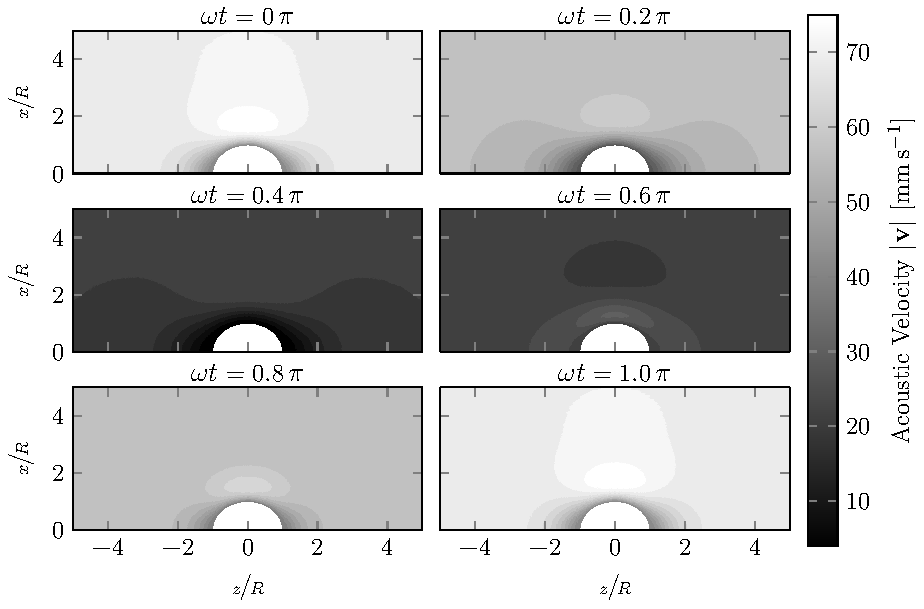
\includegraphics[]{/SC_mode1.pdf}
    \label{fig:TA-SC_mode1}
  \end{subfigure}
  \caption{First order absolute fluid velocity field at different time steps. 
  For both plots the same scaling applies. a) all modes up to $n=5$; b) single 
  mode for $n=1$. Material properties for the particle and the fluid are given 
in \cref{tab:TA-parameters}. The plotted data is generated with the Python 
module \emph{osaft}~\cite{Fankhauser2022}.}
  \label{fig:TA-SC}
\end{figure}

With the solution to the constants $\alpha_{n}$ and $\beta_{n}$ the first order 
velocity field for a rigid spherical particle and a viscous fluid is solved. 
The field inside the particle has the same magnitude and direction for all 
points because the particle is modeled rigid and therefore it is only able to 
perform rigid-body motion. The rigid-body mode in the multipole expansion is 
the dipole mode ($n=1$). Since the boundary conditions enforce a matching 
velocity at the particle-fluid interface, the whole first order fluid velocity 
solution is also dominated by that mode. This is also depicted in 
\cref{fig:TA-SC} where the fluid velocity for water and a silicium dioxide 
particle (\SiO) for the sum of all modes through $n=5$ and the fluid velocity 
only of the first mode $n=1$ is computed. \Cref{fig:TA-SC_all} and 
\Cref{fig:TA-SC_mode1} are indistinguishable from each other meaning that the 
solution to the whole first order velocity field is due to the rigid-body mode 
in the multipole expansion.

\section{Second Order Solution\label{sec:TA-secondorder}}

Similar to the first order equations one can collect all terms up to second 
order. The general mass conservation (\cref{eq:TA-massconservation}) transforms 
to
\begin{equation}
  \pdv{\ndOrder{\density}}{t} + \pdv{x_{i}}\left(\stOrder{\density}\,\stOrder{\vel_{i}} 
  + \zeOrder{\density}\,\ndOrder{\vel_{i}} \right) = 0
  \label{eq:TA-nd-massconservatio}
\end{equation}
and the second order Navier-Stokes (\cref{eq:TA-navierconservative}) becomes
\begin{equation}
  \stOrder{\density}\,\pdv{\stOrder{\vel_{i}}}{t} + \zeOrder{\density} 
  \pdv{\ndOrder{\vel_{i}}}{t} + 
  \zeOrder{\density}\,\stOrder{\vel_{j}}\,\pdv{\stOrder{\vel_{j}}}{x_{j}} = 
  \pdv{\ndOrder{\stress}}{x_{j}}
  \label{eq:TA-nd-navier}
\end{equation}
where the second order stress tensor (\cref{eq:TA-stress}) is
\begin{equation}
  \ndOrder{\stress} = \muef\left[ \pdv{\ndOrder{\vel_{i}}}{x_{j}} + 
  \pdv{\ndOrder{\vel_{j}}}{x_{i}} \right] + \left[ \mu_{\MR{B}} - 
  \frac{2}{3}\,\muef \right] \pdv{\ndOrder{\vel_{k}}}{x_{k}} \,\delta_{ij} - 
  \ndOrder{\pre}\,\delta_{ij}.
  \label{eq:TA-nd-stress}
\end{equation}

For the second order velocity field one is usually interested in the 
time-average of this field. This steady-state is referred to as AS field. 
Applying the time-average to \cref{eq:TA-nd-massconservatio,eq:TA-nd-navier} 
and using the property that the time-average of the time-derivative of a 
bounded, differentiable function is zero~\cite{Baasch2020}
\begin{equation}
  \timeaverage{\pdv{t}\,g(\vb{x};t)} = \lim\limits_{\tau \rightarrow T}{\,
    \left[ \frac{1}{\tau}\,\left( g(\vb{x}; \tau) - g(\vb{x}; 0) \right) 
  \right]} = 0,
  \label{eq:TA-avg-property}
\end{equation}
one can simplify the second order mass conservation and second order 
Navier-Stokes equation further to
\begin{equation}
  \pdv{x_{i}}\left( \timeaverage{\ndOrder{\vel_{i}}} \right) = 
  -\frac{1}{\zeOrder{\density}} \pdv{x_{i}}\left(\timeaverage{ 
  \stOrder{\density}\,\stOrder{\vel_{i}} }\right)
  \label{eq:TA-avg-massconservatio}
\end{equation}
and
\begin{equation}
  \timeaverage{\stOrder{\density} \pdv{\stOrder{\vel_{i}}}{t}} + 
  \zeOrder{\density}\,\timeaverage{\stOrder{\vel_{j}}\,\pdv{\stOrder{\vel_{j}}}{x_{j}}} 
  = \pdv{x_{j}}\left( \timeaverage{\ndOrder{\stress}} \right).
  \label{eq:TA-avg-navier}
\end{equation}

Note here, that the first term on the left hand side of \cref{eq:TA-avg-navier} 
does not vanish. Taking the partial time derivative of the time-averaged 
product of the two first order fields 
$\left(\stOrder{\density}\,\stOrder{\vel_{i}}\right)$
\begin{equation}
  \timeaverage{\pdv{t}\left( \stOrder{\density}\,\stOrder{\vel_{i}} \right)}
  =
  \timeaverage{\stOrder{\vel_{i}}\,\pdv{\stOrder{\density}}{t}}
  +
  \timeaverage{\stOrder{\density}\,\pdv{\stOrder{\vel_{i}}}{t}}
\end{equation}
and re-arranging it to
\begin{equation}
  \timeaverage{\stOrder{\density}\,\pdv{\stOrder{\vel_{i}}}{t}}
  =
  \underbrace{
  \timeaverage{\pdv{t}\left( \stOrder{\density}\,\stOrder{\vel_{i}} \right)}
}_{=0}
  -
  \underbrace{
  \timeaverage{\stOrder{\vel_{i}}\,\pdv{\stOrder{\density}}{t}}
}_{\neq 0}
  \label{eq:TA-non-zero-term}
\end{equation}
reveals that the first term on the right hand side of 
\cref{eq:TA-non-zero-term} vanishes because of the property explained in 
\cref{eq:TA-avg-property} and the second term is non-zero.

As for the first order field, the second order velocity can be decomposed into 
a sum of a streaming velocity driven solely by the known incident field and an 
unknown streaming velocity due to the scattered field
\begin{equation}
  \timeaverage{\ndOrder{\vel_{i}}} =
    \timeaverage{\ndOrder{\vel_{i,\MR{in}}}} +
    \timeaverage{\ndOrder{\vel_{i,\MR{sc}}}}.
  \label{eq:TA-nd-velocity}
\end{equation}

The time-averaged second order incident field 
$\timeaverage{\ndOrder{\vel_{i,\MR{in}}}}$ is the time-averaged motion of the 
fluid without particle. For our assumption of a spherical particle in an 
unbounded fluid, this type of AS is called \emph{Eckart streaming} named after 
\cname{Eckart1948} who derived it for the first time. However, this type of AS 
is uncommon in MSAF devices because the fluid is always in some kind of a 
cavity. The AS pattern that usually appears in MSAF devices is a combination of 
\emph{Schlichting streaming} at the fluid-structure interface and 
\emph{Rayleigh streaming} in the bulk of the fluid. Rayleigh streaming is 
driven by the boundary near Schlichting streaming. This interaction of the two 
streaming fields is named after \cname{Schlichting1932} and 
\cname{Rayleigh1894}, respectively, and qualitatively depicted in 
\cref{fig:TA-acoustic_streaming} for a plane standing pressure wave with a 
single pressure nodal plane. Note here, that this interaction can also occur at 
the particle-fluid interface. Depending on the material parameter of the fluid 
and the particle, the streaming contribution around the particle can become 
large enough and substantially contribute to the total acoustic 
force~\cite{Baasch2019}. In order to visualize any of the mentioned streaming 
fields, one needs to perform a numerical simulation and solve for the 
time-averaged fields.


\begin{figure}[tbp]
  \centering
  % \tikzsetnextfilename{acoustic_streaming}
{\small
% Parameters for vector
\pgfmathsetmacro{\W}{12.0}
\pgfmathsetmacro{\H}{6.0}
\pgfmathsetmacro{\B}{0.5}

\pgfmathsetmacro{\d}{1.1}

\pgfmathsetmacro{\fac}{0.5}
\pgfmathsetmacro{\amplitude}{1.8}
\pgfmathsetmacro{\doublefac}{2*\fac}

% Syntax: [draw options] (center) (initial angle:final angle:radius)
\def\centerarc[#1](#2)(#3:#4:#5)
  { \draw[#1] ($(#2)+({#5*cos(#3)},{#5*sin(#3)})$) arc (#3:#4:#5); }

\newcommand{\leftstreaming}[4]{
  \draw[-latex] (#1,#2) ellipse (0.9*\W/4 and 0.4*#4);

  \draw[ultra thick, #3, -latex] (#1,#2) [partial ellipse=205:285:0.9*\W/4 and 
  0.4*#4];
  \draw[ultra thick, #3, -latex] (#1,#2) [partial ellipse=305:425:0.9*\W/4 and 
  0.4*#4];
  \draw[ultra thick, #3, -latex] (#1,#2) [partial ellipse=435:515:0.9*\W/4 and 
  0.4*#4];
}

\newcommand{\rightstreaming}[4]{
  \draw[-latex] (#1,#2) ellipse (0.9*\W/4 and 0.4*#4);
  \draw[ultra thick, #3, -latex] (#1,#2) [partial ellipse=105:25:0.9*\W/4 and 
  0.4*#4];
  \draw[ultra thick, #3, -latex] (#1,#2) [partial ellipse=225:125:0.9*\W/4 and 
  0.4*#4];
  \draw[ultra thick, #3, -latex] (#1,#2) [partial ellipse=345:255:0.9*\W/4 and 
  0.4*#4];
}

\newcommand{\streamingOne}[4]{
  \leftstreaming{#1}{#2}{#3}{#4}
  \rightstreaming{#1+\W/2}{#2}{#3}{#4}
}

\newcommand{\streamingTwo}[4]{
  \rightstreaming{#1}{#2}{#3}{#4}
  \leftstreaming{#1+\W/2}{#2}{#3}{#4}
}


\begin{tikzpicture}[]

  \coordinate (O) at (0,0);
  \coordinate (BL) at (-\W/2,-\H/2);
  \coordinate (TR) at (\W/2,\H/2);

  % walls
  \draw[pattern=north west lines, pattern color=black!50] ($(BL) - (\B, 
  \B)$) rectangle ++(2*\B+\W,2*\B+\H);

  % fluid
  \draw[fill=blue!10] (BL) rectangle (TR);
  % boundary layer
  \path[fill=blue!20] (BL) rectangle ($(BL) + (\W,\d)$);
  \path[fill=blue!20] (TR) rectangle ($(TR) - (\W,\d)$);


  % coordinate system
  \draw[<->] ($(-\W/2*0.9,-\H/4)$) -- node[left,pos=0] {$\ez$} ++(0,-\H/4*0.9) 
  -- node[above,pos=1] {$\ey$} ++(\H/7,0);

  % pressure field
  \draw[blue] plot[domain=-\W/2:\W/2,samples=100] 
  (\x,{+\amplitude*sin(deg(2*pi/(\W/\fac)*\x))});
  \draw[blue] plot[domain=-\W/2:\W/2,samples=100] 
  (\x,{-\amplitude*sin(deg(2*pi/(\W/\fac)*\x))});


  % annotations width
  \draw[|<->|] (-\W/2, \H/2+1.5*\B) -- node[above,midway] {$W$} ++(\W,0);
  \draw[|<->|] (\W/2+1.5*\B, -\H/2) -- node[right,midway] {$H$} ++(0,\H);

  \draw[|<->|] (-\W/2-1.5*\B, -\H/2) -- node[left,midway] {$\delta$} ++(0,\d);
  \draw[|<->|] (-\W/2-1.5*\B, +\H/2) -- node[left,midway] {$\delta$} ++(0,-\d);

  % schlichting streaming
  \streamingOne{-\W/4}{\H/2-\d/2}{red}{\d}
  \streamingTwo{-\W/4}{-\H/2+\d/2}{red}{\d}

  % rayleigh streaming
  \streamingTwo{-\W/4}{\H/4-\d/2}{olive}{\H/2-\d/3}
  \streamingOne{-\W/4}{-\H/4+\d/2}{olive}{\H/2-\d/3}
\end{tikzpicture}
}

  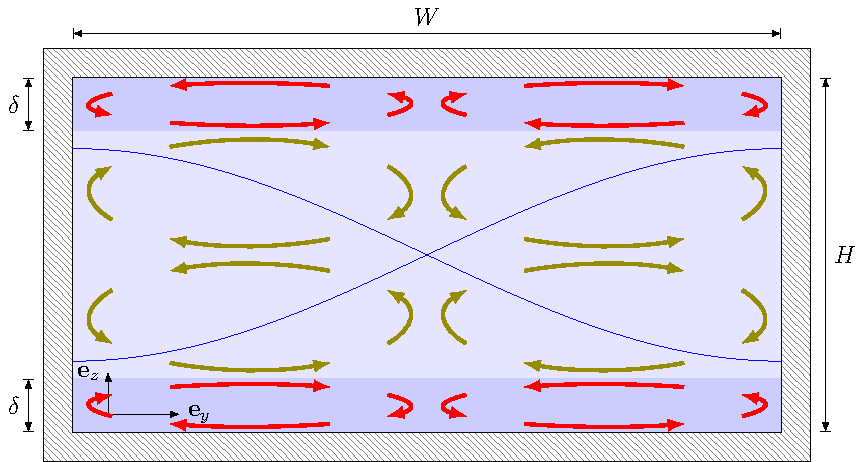
\includegraphics[]{/acoustic_streaming.pdf}
  \caption{Schlichting and Rayleigh acoustic streaming for an one-dimensional 
    standing pressure wave (\textcolor{blue}{blue line}) in a rectangular fluid 
    cavity of width $W$ and heigth $H$. Near the viscous boundary layer 
    $\delta$ (darker regions at the boundary) Schlichting streaming 
    (\textcolor{red}{red arrows}) is present and in the bulk of the fluid 
  Rayleigh acoustic streaming (\textcolor{olive}{olive arrows}).}
  \label{fig:TA-acoustic_streaming}
\end{figure}

The scattered field is -- as before -- decomposed into the gradient of a scalar 
velocity potential and the curl of a vector velocity potential
\begin{equation}
  \timeaverage{\ndOrder{\vel_{i,\MR{sc}}}} =
  \pdv{\ndOrder{\phi}}{x_{i}} + 
  \epsilon_{kli}\,\pdv{\ndOrder{\psi}_{l}}{x_{k}}.
  \label{eq:TA-nd-sc-decomposition}
\end{equation}

The boundary conditions for the time-averaged second order velocity field is 
defined at the particle-fluid interface and enforces the equality of the second 
order Eulerian velocity to the negative Stokes drift
\begin{equation}
  \timeaverage{\ndOrder{\vel_{i}}}
  =
  -
  \underbrace{
    \timeaverage{\frac{1}{-\iu\omega}\,\vel_{j}\,\pdv{\vel_{i}}{x_{j}}}
  }_{\text{Stokes drift}}
  \quad\text{at~}r=R.
  \label{eq:TA-nd-BCs}
\end{equation}


At this point we will not repeat the calculation to solve for the second order 
velocity field. Interested readers are pointed to \cname{Doinikov1994Rigid} 
Equation (4.1) through (4.34).

% \begin{figure}
  % \centering
  % \begin{subfigure}[b]{\textwidth}
    % \centering
    % \caption{Modes through $n=5$}
    % % \tikzsetnextfilename{SC_all}

\renewcommand{\tikzHelper}{\relPath/10_Figures/TikZ/scattering_data}

\begin{tikzpicture}
\begin{groupplot}[
  group style={
    vertical sep=6mm,
    horizontal sep=3mm,
    group size= 2 by 3,
  },
  title style={yshift=-2.5mm,},
  xmin=-5,
  xmax=5,
  ymin=0,
  ymax=5,
  point meta max=75,
  point meta min=4,
  view={0}{90},
  % colorbar,
  colormap = {whiteblack}{color(0cm)  = (black);color(1cm) = (white)},
  % colormap/bluered,                     % Colormap preset
  height=4cm,
  width=75mm,
  ]

  %%%%%%%%%%%%%%%%
  \nextgroupplot[
    title={$\omega t =0\,\pi$},
    ylabel={$\sfrac{x}{R}$},
    xticklabels={,,},
]
    \addplot3[
        contour filled={number=25,labels={false}},
        mesh/rows=110,
        mesh/check=false
    ] table[x=z, y=x, z=c] {\tikzHelper/phase_0.dat};

    \coordinate (top) at (rel axis cs:0,1);
  %%%%%%%%%%%%%%%%
  \nextgroupplot[
    title={$\omega t =0.2\,\pi$},
    xticklabels={,,},
    yticklabels={,,},
]
    \addplot3[
        contour filled={number=25,labels={false}},
        mesh/rows=110,
        mesh/check=false
    ] table[x=z, y=x, z=c] {\tikzHelper/phase_1.dat};

  %%%%%%%%%%%%%%%%
  \nextgroupplot[
    title={$\omega t =0.4\,\pi$},
    ylabel={$\sfrac{x}{R}$},
    xticklabels={,,},
]
    \addplot3[
        contour filled={number=25,labels={false}},
        mesh/rows=110,
        mesh/check=false
    ] table[x=z, y=x, z=c] {\tikzHelper/phase_2.dat};

  %%%%%%%%%%%%%%%%
  \nextgroupplot[
    title={$\omega t =0.6\,\pi$},
    xticklabels={,,},
    yticklabels={,,},
]
    \addplot3[
        contour filled={number=25,labels={false}},
        mesh/rows=110,
        mesh/check=false
    ] table[x=z, y=x, z=c] {\tikzHelper/phase_3.dat};

  %%%%%%%%%%%%%%%%
  \nextgroupplot[
    title={$\omega t =0.8\,\pi$},
    ylabel={$\sfrac{x}{R}$},
    xlabel={$\sfrac{z}{R}$},
]
    \addplot3[
        contour filled={number=25,labels={false}},
        mesh/rows=110,
        mesh/check=false
    ] table[x=z, y=x, z=c] {\tikzHelper/phase_4.dat};

  %%%%%%%%%%%%%%%%
  \nextgroupplot[
    title={$\omega t =1.0\,\pi$},
    yticklabels={,,},
    xlabel={$\sfrac{z}{R}$},
]
    \addplot3[
        contour filled={number=25,labels={false}},
        mesh/rows=110,
        mesh/check=false
    ] table[x=z, y=x, z=c] {\tikzHelper/phase_5.dat};

  \coordinate (bot) at (rel axis cs:1,0);

\end{groupplot}
  \path (top-|current bounding box.east)--
                    coordinate(legendposright)
                    (bot-|current bounding box.east);


\begin{axis}[%
  hide axis,
  scale only axis,
  %height=0.975\linewidth,
  %width=0.01\linewidth,
  at={(legendposright.east)},
  anchor=east,
  xshift=60mm,
  point meta min=4.0,
  point meta max=75.0,
  % colormap/bluered,                     % Colormap preset
  colormap = {whiteblack}{color(0cm)  = (black);color(1cm) = (white)},
  colorbar right,                  % Active colorbar
  colorbar sampled,                     % Steps in colorbar
  colorbar style={
    separate axis lines,
    samples=256,                        % Number of steps
    ylabel={Acoustic Velocity $\abs{\vb{v}}$ [\si{\mm\per\second}]},
  },
  every colorbar/.append style={
    height=\pgfkeysvalueof{/pgfplots/parent axis height}%+
               %\pgfkeysvalueof{/pgfplots/group/vertical sep}
  }
]
  \addplot [draw=none] coordinates {(0,0)};
\end{axis}

\end{tikzpicture}

    % % 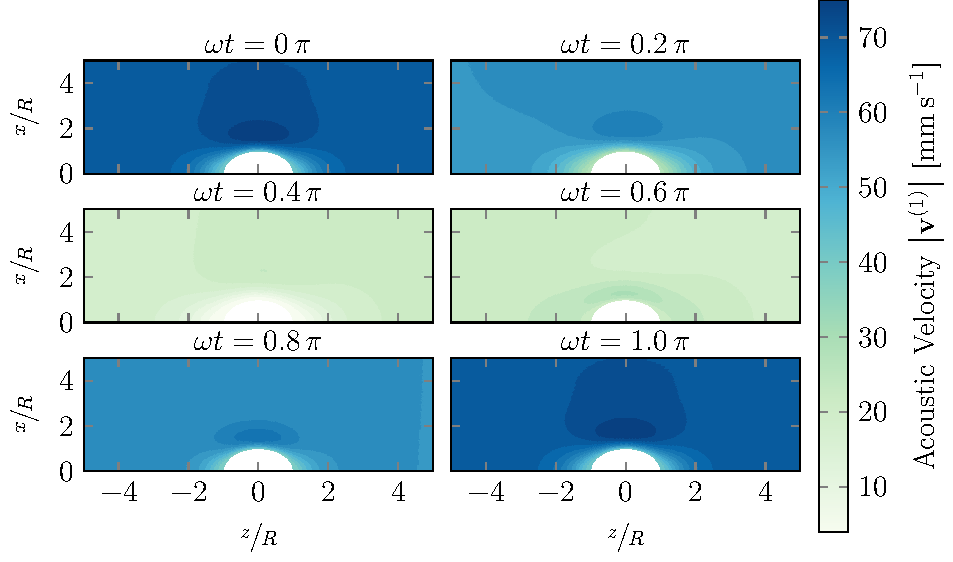
\includegraphics[]{/SC_all.pdf}
    % \includegraphics[width=100mm]{example-image-a}
    % % \label{fig:TA-SC_all}
  % \end{subfigure}\\%
  % \begin{subfigure}[b]{\textwidth}
    % \centering
    % \caption{Single mode one $n=1$}
    % % \tikzsetnextfilename{SC_mode1}

\renewcommand{\tikzHelper}{\relPath/10_Figures/TikZ/scattering_data}

\begin{tikzpicture}
\begin{groupplot}[
  group style={
    vertical sep=6mm,
    horizontal sep=3mm,
    group size= 2 by 3,
  },
  title style={yshift=-2.5mm,},
  xmin=-5,
  xmax=5,
  ymin=0,
  ymax=5,
  point meta max=75,
  point meta min=4,
  view={0}{90},
  % colorbar,
  colormap = {whiteblack}{color(0cm)  = (black);color(1cm) = (white)},
  % colormap/bluered,                     % Colormap preset
  height=4cm,
  width=75mm,
  ]

  %%%%%%%%%%%%%%%%
  \nextgroupplot[
    title={$\omega t =0\,\pi$},
    ylabel={$\sfrac{x}{R}$},
    xticklabels={,,},
]
    \addplot3[
        contour filled={number=25,labels={false}},
        mesh/rows=110,
        mesh/check=false
    ] table[x=z, y=x, z=c] {\tikzHelper/phase_0_mode_1.dat};

    \coordinate (top) at (rel axis cs:0,1);
  %%%%%%%%%%%%%%%%
  \nextgroupplot[
    title={$\omega t =0.2\,\pi$},
    xticklabels={,,},
    yticklabels={,,},
]
    \addplot3[
        contour filled={number=25,labels={false}},
        mesh/rows=110,
        mesh/check=false
    ] table[x=z, y=x, z=c] {\tikzHelper/phase_1_mode_1.dat};

  %%%%%%%%%%%%%%%%
  \nextgroupplot[
    title={$\omega t =0.4\,\pi$},
    ylabel={$\sfrac{x}{R}$},
    xticklabels={,,},
]
    \addplot3[
        contour filled={number=25,labels={false}},
        mesh/rows=110,
        mesh/check=false
    ] table[x=z, y=x, z=c] {\tikzHelper/phase_2_mode_1.dat};

  %%%%%%%%%%%%%%%%
  \nextgroupplot[
    title={$\omega t =0.6\,\pi$},
    xticklabels={,,},
    yticklabels={,,},
]
    \addplot3[
        contour filled={number=25,labels={false}},
        mesh/rows=110,
        mesh/check=false
    ] table[x=z, y=x, z=c] {\tikzHelper/phase_3_mode_1.dat};

  %%%%%%%%%%%%%%%%
  \nextgroupplot[
    title={$\omega t =0.8\,\pi$},
    ylabel={$\sfrac{x}{R}$},
    xlabel={$\sfrac{z}{R}$},
]
    \addplot3[
        contour filled={number=25,labels={false}},
        mesh/rows=110,
        mesh/check=false
    ] table[x=z, y=x, z=c] {\tikzHelper/phase_4_mode_1.dat};

  %%%%%%%%%%%%%%%%
  \nextgroupplot[
    title={$\omega t =1.0\,\pi$},
    yticklabels={,,},
    xlabel={$\sfrac{z}{R}$},
]
    \addplot3[
        contour filled={number=25,labels={false}},
        mesh/rows=110,
        mesh/check=false
    ] table[x=z, y=x, z=c] {\tikzHelper/phase_5_mode_1.dat};

  \coordinate (bot) at (rel axis cs:1,0);

\end{groupplot}
  \path (top-|current bounding box.east)--
                    coordinate(legendposright)
                    (bot-|current bounding box.east);


\begin{axis}[%
  hide axis,
  scale only axis,
  %height=0.975\linewidth,
  %width=0.01\linewidth,
  at={(legendposright.east)},
  anchor=east,
  xshift=60mm,
  point meta min=4.0,
  point meta max=75.0,
  % colormap/bluered,                     % Colormap preset
  colormap = {whiteblack}{color(0cm)  = (black);color(1cm) = (white)},
  colorbar right,                  % Active colorbar
  colorbar sampled,                     % Steps in colorbar
  colorbar style={
    separate axis lines,
    samples=256,                        % Number of steps
    ylabel={Acoustic Velocity $\abs{\stOrder{\vb{v}}}$ [\si{\mm\per\second}]},
  },
  every colorbar/.append style={
    height=\pgfkeysvalueof{/pgfplots/parent axis height}%+
               %\pgfkeysvalueof{/pgfplots/group/vertical sep}
  }
]
  \addplot [draw=none] coordinates {(0,0)};
\end{axis}

\end{tikzpicture}

    % % 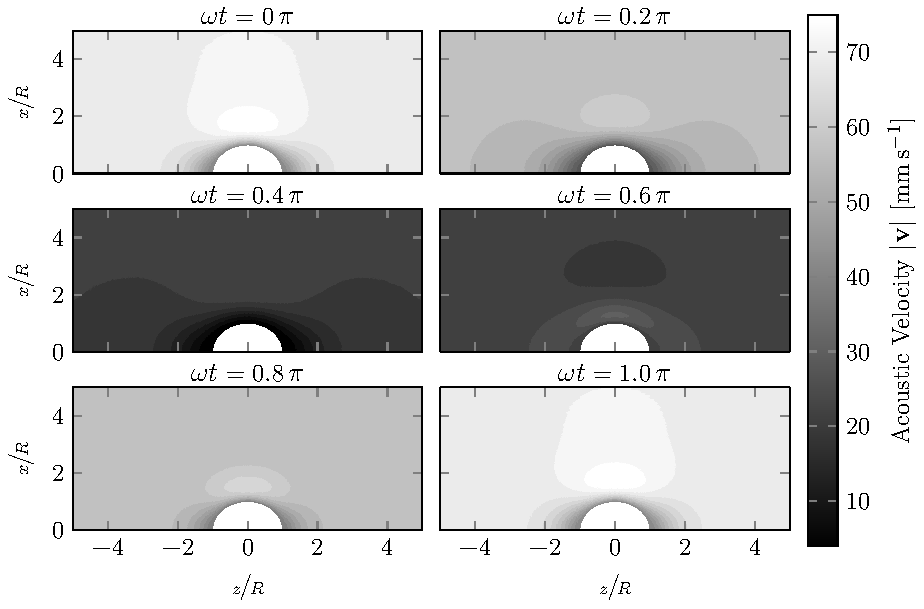
\includegraphics[]{/SC_mode1.pdf}
    % \includegraphics[width=100mm]{example-image-b}
    % % \label{fig:TA-SC_mode1}
  % \end{subfigure}
  % \caption{First order fluid velocity field at different steps during one 
% period. For both plots the same scaling applies. a) all modes through $n=5$; 
% b) single mode one for $n=1$. Material properties for the particle and the 
% fluid are seen in \cref{tab:TA-parameters,tab:TC-parameters}. The plotted data 
% is generated with the Python module \emph{osaft}~\cite{FankhauserPython2022}.}
  % \label{fig:TA-AS}
% \end{figure}

% \textcolor{red}{in \cref{fig:TA-AS} yo can asee bloah balh the time averaged 
% streaming field around the particle for}

This time-averaged streaming field causes a force onto the particle in the 
direction of the flow which is known as Stokes' drag force
\begin{equation}
  \force^{\MR{drag}}_{i} = \gamma\,\timeaverage{\ndOrder{\vel_{i}}} = 
  6\pi\,R\,\muef\,
  \left( \timeaverage{\ndOrder{\vel_{i}}} - \vel_{i,\MR{p}} \right)
  \label{eq:TA-drag-force}
\end{equation}
where $\gamma$ is also called Stokes' drag coefficient and $\vel_{i,\MR{p}}$ 
the particle velocity.


\section{Acoustic Radiation Force\label{sec:TA-ARF}}

With the solution for the first and second order velocity field and hence for 
the stress tensors of the respective orders one can calculate the ARF with 
\cref{eq:TA-def-approx-ARF}. However, this formula and also the velocity fields 
are cumbersome to compute. It is cumbersome because the formula of 
\cname{Doinikov1994Rigid} as well as the solutions to the velocity fields are 
valid for any axisymmetric incident acoustic wave field and are not restricted 
to the ratios of the particle radius to the VBL thickness $\sfrac{R}{\delta}$, 
the ratio of the particle radius to the acoustic wavelength 
$\sfrac{R}{\wavelength_{\MR{a}}} = \sfrac{(\R\fex)}{\cfl}$, and the ratio of 
the VBL thickness to the acoustic wavelength 
$\sfrac{\delta}{\wavelength_{\MR{a}}}$.

\begin{figure}[tbp]
  \centering
  % \tikzsetnextfilename{lambda_mode}
% Parameters for vector
\pgfmathsetmacro{\W}{8.0}
\pgfmathsetmacro{\Wrect}{1.0}
\pgfmathsetmacro{\Hrect}{3.0}

\pgfmathsetmacro{\freq}{pi/4}

\pgfmathsetmacro{\xpOne}{\freq/pi*\W}
\pgfmathsetmacro{\xpTwo}{\freq/pi*\W+\W/2}

\begin{tikzpicture}[]

  \coordinate (O) at (0,0);
  \coordinate (TL) at (\W,\Hrect);

  % coordinate system

  \draw[<->] ($(-\Wrect*1.5,\Hrect/2)$) -- node[left,pos=0] {$\ez$} 
  ++(0,-\Hrect/1.7) -- node[right,pos=1] {$\ey$} ++(\Hrect/2,0);

  % fluid
  \fill[blue!10] (O) rectangle (TL);

  % middle line
  \draw[black, thick, dotted] ($(O) + (0,\Hrect/2)$) -- ++(\W,0);

  % nodal planes
  \draw[black, dotted] ($(\xpOne,\Hrect/2)$) -- ++(0,\Hrect/2);
  \draw[black, dotted] ($(\xpTwo,\Hrect/2)$) -- ++(0,\Hrect/2);


  % walls
  \draw[pattern=north west lines, pattern color=black!50] (0,0) rectangle 
  ++(-\Wrect,\Hrect);
  \draw[pattern=north west lines, pattern color=black!50] (\W,0) rectangle 
  ++(\Wrect,\Hrect);

  % pressure
  \draw[blue] plot[domain=0:\W,samples=100] (\x,{cos(deg(\freq*\x))+\Hrect/2});
  \draw[blue] plot[domain=0:\W,samples=100] 
  (\x,{-cos(deg(\freq*\x))+\Hrect/2});

  % force field
  % \draw[red, dashdotted] plot[domain=0:\W,samples=100] 
  % (\x,{sin(deg(2*\freq*\x))+\Hrect/2});

  % particles
  \node[shade,shading=ball,circle,ball color=black!50!white,minimum size=3mm] 
  (positive) at  (\xpOne,\Hrect/3) {};
  \node[shade,shading=ball,circle,ball color=black!50!white,minimum size=3mm] 
  (positivetwo) at  (\xpTwo,\Hrect/4) {};

  \node[shade,shading=ball,circle,ball color=red!50!white,minimum size=2mm] 
  (negative) at  (\W/2,\Hrect*2/3) {};

  % annotations width
  \draw[|<->|] ($(O) - (0,0.8)$) -- node[above,midway] {$W$} ++(\W,0);
  % annotations pressure field
  \draw[|<->|] ($(\xpOne,\Hrect)+ (0,0.5)$) -- node[above,midway] 
  {$\sfrac{\lambda_{\mathrm{a}}}{2}$} ++($(\W/2,0)$);
  % annotations positive
  \draw[thin,-](positive) to[out=-130, in=180] ++(-0.5,-0.7)
      node[right] {$\Phi > 0$};
  \draw[thin,-](positivetwo) to[out=300, in=180] ++(0.2,-0.4)
      node[right] {$\Phi > 0$};
  % annotations positive
  \draw[-, thin] (negative) to[out=120, in=180] ++(-0.5,0.8)
  node[right] {$\Phi < 0$};



\end{tikzpicture}

  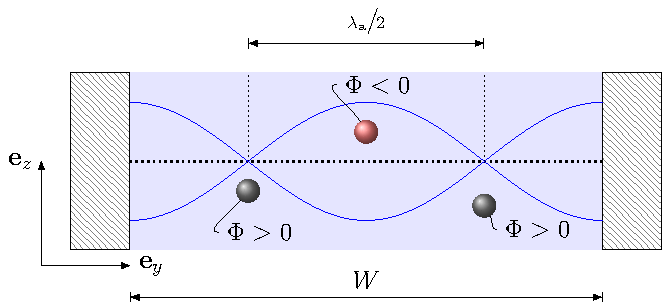
\includegraphics[]{/lambda_mode.pdf}
  \caption{Sketch of one-dimensional standing pressure wave (blue line) in a 
      fluid cavity with width $W$, an acoustic wavelength 
      $\wavelength_{\MR{a}}$, and two types of particle; red (negative contrast 
      factor $\Phi$), gray (positive contrast factor $\Phi$). The depicted mode 
    is the $\lambda$-mode.}
  \label{fig:TA-lambda_mode}
\end{figure}

But for most applications, firstly, the particle radius is much larger than the 
VBL thickness $R \gg \delta$ and, secondly, the acoustic wavelength is much 
larger than the particle radius $\wavelength_{\MR{a}}\gg R \gg \delta$. This 
special parameter regime is sill included in the solution of 
\cname{Doinikov1994Rigid}, however, there exist an easier formula for this 
regime. The most common formula for those restrictions and an one-dimensional 
standing pressure wave is the derivation by \cname{Gorkov1962}. He derives the 
ARF on a particle which is much smaller than the acoustic wavelength 
($\R\ll\lambda_{\MR{a}}$). In his derivations, he models the fluid as well as 
the particle as an inviscid compressible fluid. The assumption of an inviscid 
fluid for the particle is extending \cname{Doinikov1994Rigid} assumption of an 
rigid particle. Since the fluid is also modeled as an inviscid fluid, no VBL 
can be formed. The ARF is defined as the negative gradient of a potential
\begin{equation}
  \force^{\MR{rad}}_{i} = -\pdv{x_{i}}U^{\MR{rad}}
  \label{eq:TA-gorkov}
\end{equation}
where $U^{\MR{rad}}$ is the so-called \emph{Gor'kov potential}. It is defined 
as
\begin{equation}
  U^{\MR{rad}} = \frac{4}{3}\,\pi\,R^{3}\left\{ 
  \frac{f_{1}}{2}\,\kappa_{\MR{f}}\timeaverage{p^{2}_{\MR{a}}} - 
f_{2}\,\rhof\timeaverage{v^{2}_{i,\MR{in}}} \right\}
    \label{eq:TA-gorkov-potential}
\end{equation}
where $\kappa_{\MR{f}}$ is the compressibility of the fluid and the so-called 
monopole factor
\begin{equation}
  f_{1} = 1 - \frac{\kappa_{\MR{s}}}{\kappa_{\MR{f}}} = 1 - \tilde{\kappa}
  \label{eq:TA-fone}
\end{equation}
with $\kappa_{\MR{s}}$ being the compressibility of the particle and where
\begin{equation}
f_{2} = \frac{2(\tilde{\rho}-1)}{2\tilde{\rho}+1}
\label{eq:TA-ftwo}
\end{equation}
is the so called dipole factor with $\tilde{\rho} = \sfrac{\rhop}{\rhof}$ 
\cite{Gorkov1962,Bruus2012}.

% \begin{figure}
    % % \tikzsetnextfilename{SC_all}

\renewcommand{\tikzHelper}{\relPath/10_Figures/TikZ/scattering_data}

\begin{tikzpicture}
\begin{groupplot}[
  group style={
    vertical sep=6mm,
    horizontal sep=3mm,
    group size= 2 by 3,
  },
  title style={yshift=-2.5mm,},
  xmin=-5,
  xmax=5,
  ymin=0,
  ymax=5,
  point meta max=75,
  point meta min=4,
  view={0}{90},
  % colorbar,
  colormap = {whiteblack}{color(0cm)  = (black);color(1cm) = (white)},
  % colormap/bluered,                     % Colormap preset
  height=4cm,
  width=75mm,
  ]

  %%%%%%%%%%%%%%%%
  \nextgroupplot[
    title={$\omega t =0\,\pi$},
    ylabel={$\sfrac{x}{R}$},
    xticklabels={,,},
]
    \addplot3[
        contour filled={number=25,labels={false}},
        mesh/rows=110,
        mesh/check=false
    ] table[x=z, y=x, z=c] {\tikzHelper/phase_0.dat};

    \coordinate (top) at (rel axis cs:0,1);
  %%%%%%%%%%%%%%%%
  \nextgroupplot[
    title={$\omega t =0.2\,\pi$},
    xticklabels={,,},
    yticklabels={,,},
]
    \addplot3[
        contour filled={number=25,labels={false}},
        mesh/rows=110,
        mesh/check=false
    ] table[x=z, y=x, z=c] {\tikzHelper/phase_1.dat};

  %%%%%%%%%%%%%%%%
  \nextgroupplot[
    title={$\omega t =0.4\,\pi$},
    ylabel={$\sfrac{x}{R}$},
    xticklabels={,,},
]
    \addplot3[
        contour filled={number=25,labels={false}},
        mesh/rows=110,
        mesh/check=false
    ] table[x=z, y=x, z=c] {\tikzHelper/phase_2.dat};

  %%%%%%%%%%%%%%%%
  \nextgroupplot[
    title={$\omega t =0.6\,\pi$},
    xticklabels={,,},
    yticklabels={,,},
]
    \addplot3[
        contour filled={number=25,labels={false}},
        mesh/rows=110,
        mesh/check=false
    ] table[x=z, y=x, z=c] {\tikzHelper/phase_3.dat};

  %%%%%%%%%%%%%%%%
  \nextgroupplot[
    title={$\omega t =0.8\,\pi$},
    ylabel={$\sfrac{x}{R}$},
    xlabel={$\sfrac{z}{R}$},
]
    \addplot3[
        contour filled={number=25,labels={false}},
        mesh/rows=110,
        mesh/check=false
    ] table[x=z, y=x, z=c] {\tikzHelper/phase_4.dat};

  %%%%%%%%%%%%%%%%
  \nextgroupplot[
    title={$\omega t =1.0\,\pi$},
    yticklabels={,,},
    xlabel={$\sfrac{z}{R}$},
]
    \addplot3[
        contour filled={number=25,labels={false}},
        mesh/rows=110,
        mesh/check=false
    ] table[x=z, y=x, z=c] {\tikzHelper/phase_5.dat};

  \coordinate (bot) at (rel axis cs:1,0);

\end{groupplot}
  \path (top-|current bounding box.east)--
                    coordinate(legendposright)
                    (bot-|current bounding box.east);


\begin{axis}[%
  hide axis,
  scale only axis,
  %height=0.975\linewidth,
  %width=0.01\linewidth,
  at={(legendposright.east)},
  anchor=east,
  xshift=60mm,
  point meta min=4.0,
  point meta max=75.0,
  % colormap/bluered,                     % Colormap preset
  colormap = {whiteblack}{color(0cm)  = (black);color(1cm) = (white)},
  colorbar right,                  % Active colorbar
  colorbar sampled,                     % Steps in colorbar
  colorbar style={
    separate axis lines,
    samples=256,                        % Number of steps
    ylabel={Acoustic Velocity $\abs{\vb{v}}$ [\si{\mm\per\second}]},
  },
  every colorbar/.append style={
    height=\pgfkeysvalueof{/pgfplots/parent axis height}%+
               %\pgfkeysvalueof{/pgfplots/group/vertical sep}
  }
]
  \addplot [draw=none] coordinates {(0,0)};
\end{axis}

\end{tikzpicture}

    % % 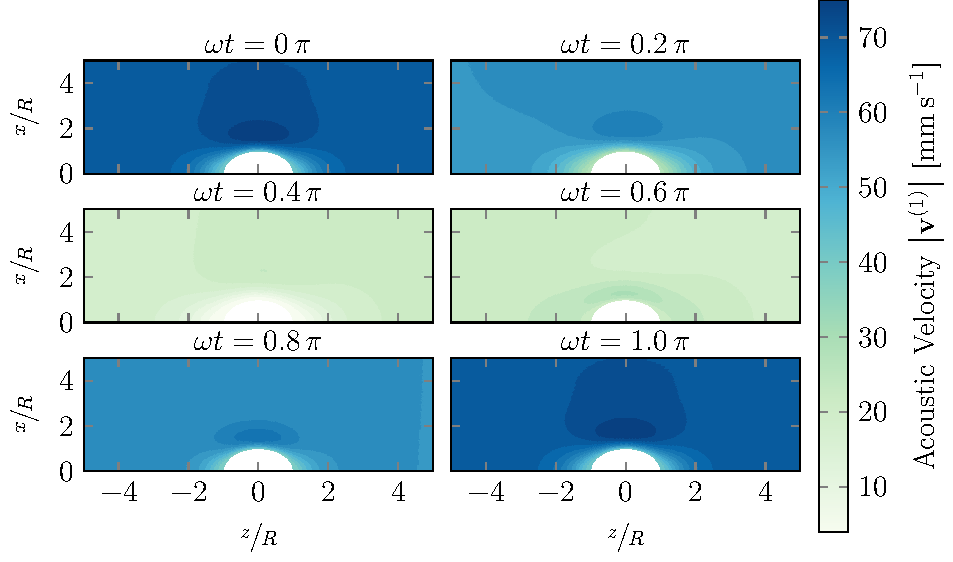
\includegraphics[]{/SC_all.pdf}
    % \includegraphics[width=160mm]{example-image-a}
    % \caption{ARF solution generated with \emph{gorkov}}
  % \label{fig:TA-comparision-ARF}
% \end{figure}

For a plane standing wave, where the wave vector is aligned with $\ez$, (see 
\cref{fig:TA-plane_wave}) the radiation force along the $\ez$ axis can be 
computed as~\cite{Bruus2012}
\begin{equation}
  \force_{z}^{\MR{rad}} = 
  4\pi\,\Phi(\tilde{\rho},\tilde{\kappa})\,k\,R^{3}\,E_{\MR{ac}}\,\sin(2kz)
  \label{eq:TA-ARFy}
\end{equation}
where $z$ denotes the position along $\ez$ and with the so called acoustic 
energy density
\begin{equation}
  E_{\MR{ac}} = \frac{p_{\MR{a}}^{2}}{4\rhof\cfl^{2}}
  \label{eq:TA-Eac}
\end{equation}
and with the so-called acoustic contrast factor
\begin{equation}
  \Phi(\tilde{\rho},\tilde{\kappa}) = \frac{1}{3}\,f_{1} + \frac{1}{2}\,f_{2}.
  \label{eq:TA-Phi}
\end{equation}

From \cref{eq:TA-ARFy} one can deduce the following interesting properties of 
the ARF for a plane standing wave: a) the ARF scales with the volume of the 
spherical particle; b) the ARF is sinusoidal with double the period of the 
incident acoustic wave; c) depending on the sign of $\Phi(\tilde{\kappa}, 
\tilde{\rho})$ the ARF changes the sign; d) particles with 
$\Phi(\tilde{\kappa}, \tilde{\rho}) = 0$ are acoustically 
$\wavelength_{\MR{a}}$
\emph{invisible} and not affected by the ARF.

Particles with a positive acoustic contrast factor $\Phi(\tilde{\kappa}, 
\tilde{\rho}) > 0$ are displaced by the ARF towards the pressure nodes (gray 
particles in \cref{fig:TA-plane_wave}) and particles with a negative acoustic 
contrast factor $\Phi(\tilde{\kappa}, \tilde{\rho}) < 0$ are displaced towards 
the pressure antinode (red particle in \cref{fig:TA-plane_wave}).

% \textcolor{red}{general solyution converges to Gorkov 
% \cref{fig:TA-comparision-ARF}}


\section{Acoustic Radiation Torque\label{sec:TA-VT}}

\Cref{eq:TA-ARFy} is valid for an one-dimensional pressure wave. However, for 
the configuration of two one-dimensional pressure waves which are orthogonal to 
each other a two dimensional pressure field is formed (see 
\cref{fig:TA-viscous_torque}). With the assumption that the object dimension is 
much smaller than the acoustic wavelength of both pressure fields separately, 
the particles with positive acoustic contrast factor ( $\Phi>0$ ) will be 
displaced into the pressure nodes of the two superposing pressure waves and the 
particles with negative acoustic contrast factor in the superposed pressure 
antinodes.

\begin{figure}[tbp]
  \centering
  % \tikzsetnextfilename{viscous_torque}
{\small
% Parameters for vector
\pgfmathsetmacro{\W}{12.0}
\pgfmathsetmacro{\H}{6.0}
\pgfmathsetmacro{\B}{0.5}

\pgfmathsetmacro{\fac}{2}
\pgfmathsetmacro{\amplitude}{0.8}
\pgfmathsetmacro{\doublefac}{2*\fac}

% Syntax: [draw options] (center) (initial angle:final angle:radius)
\def\centerarc[#1](#2)(#3:#4:#5)
  { \draw[#1] ($(#2)+({#5*cos(#3)},{#5*sin(#3)})$) arc (#3:#4:#5); }

\begin{tikzpicture}[]

  \coordinate (O) at (0,0);
  \coordinate (BL) at (-\W/2,-\H/2);
  \coordinate (TR) at (\W/2,\H/2);

  % walls
  \draw[pattern=north west lines, pattern color=black!50] ($(BL) - (\B, 
  \B)$) rectangle ++(2*\B+\W,2*\B+\H);

  % fluid
  \draw[fill=blue!10] (BL) rectangle (TR);

  % coordinate system
  \draw[<->] ($(-\W/2*0.9,-\H/4)$) -- node[left,pos=0] {$\ex$} ++(0,-\H/4*0.9) 
  -- node[right,pos=1] {$\ey$} ++(\H/4,0);

  % pressure field
  \draw[blue] plot[domain=-\W/2:\W/2,samples=100] 
  (\x,{-\amplitude*cos(deg(2*pi/(\W/\fac)*\x))});
  \draw[blue] plot[domain=-\W/2:\W/2,samples=100] 
  (\x,{\amplitude*cos(deg(2*pi/(\W/\fac)*\x))});

  \draw[purple] plot[domain=-\H/2:\H/2,samples=100] 
  ({-\amplitude*cos(deg(2*pi/(\H/\fac)*\x))},\x);
  \draw[purple] plot[domain=-\H/2:\H/2,samples=100] 
  ({\amplitude*cos(deg(2*pi/(\H/\fac)*\x))},\x);

  \foreach \x in {1,2,...,\doublefac}{
    \draw[dotted] ($(-\W/2, -\H*5/8 + \x*\H/2/\fac)$) -- ++(\W,0);
    \draw[dotted] ($( -\W*5/8 + \x*\W/2/\fac,-\H/2)$) -- ++(0,\H);
  }

  % non-spherical particles
  \foreach \x in {1,2,...,\doublefac}{
  \foreach \y in {1,2,...,\doublefac}{
    \pgfmathsetmacro{\X}{-\W*5/8 + \x*\W/2/\fac}
    \pgfmathsetmacro{\Y}{-\H*5/8 + \y*\H/2/\fac}
    \pgfmathparse{360 * random()}
    \filldraw[rotate around={\pgfmathresult:(\X,\Y)}, gray, shade, 
    shading=ball, ball color=black!50!white] (\X,\Y) ellipse (2mm and 3mm);
  }
  }

  \coordinate (TL) at (-\W*3/8,\H*3/8);
  \centerarc[thick,->](TL)(30:270:6mm)
  \node at ($(TL)+(-\W/12,\H/12)$) {$\Omega\left( \zeta \right)$};


  % annotations width
  \draw[|<->|] (-\W/2, \H/2+1.5*\B) -- node[above,midway] {$W$} ++(\W,0);
  \draw[|<->|] (\W/2+1.5*\B, -\H/2) -- node[right,midway] {$H$} ++(0,\H);
  \path (-\W/2-\B,0) -- node[midway,fill=white,rounded corners] 
  {$\propto\sin(\omega t)$} ++(\B,0);

  \path (-\W/8,\H/2+\B/2) -- node[midway,fill=white,rounded corners] 
  {$\propto\sin(\omega t + \zeta)$} ++(\W/4,0);
\end{tikzpicture}
}

  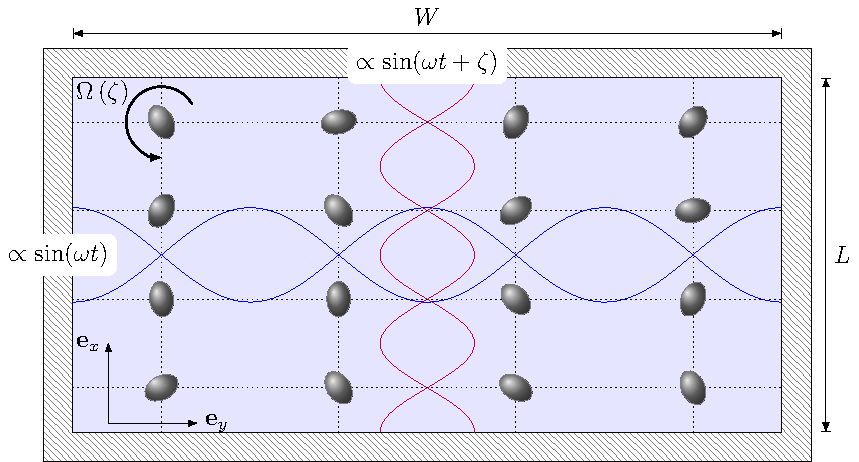
\includegraphics[]{/viscous_torque.pdf}
  \caption{Sketch of a two dimensional orthogonal pressure field in a fluid 
    cavity of width $W$ and length $L$ with phase difference $\zeta$ and 
  acoustic excitation frequency $\omega$. Particles gather in pressure nodes 
($\Phi > 0$) along respective direction. Additionally, non-spherical particles 
rotate with angular velocity $\Omega\left( \zeta \right)$.}
  \label{fig:TA-viscous_torque}
\end{figure}

Besides the translation of the objects to the equilibrium pressure position 
some of them will also rotate due to their non-spherical shape (see 
\cref{fig:TA-viscous_torque}). No analytical closed form solution exists for 
the radiation torque exerted onto the objects~\cite{Lamprecht2017}.

 % \begin{figure}
  % \centering
  % \begin{subfigure}[b]{0.35\textwidth}
    % \centering
    % \caption{$\zeta = \SI{0}{\radian}$}
    % % \tikzsetnextfilename{viscous_torque_0}

\pgfplotsset{%
    colormap={bwr}{
      color=(blue);
      color=(white);
      color=(red);
    }%
}

\begin{tikzpicture}
  \begin{axis}[view={0}{90},
      xlabel={ $\varphi$ [rad] },
      ylabel={Period  $t\cdot f$ [-]},
      xtick={0,3.1415,6.28},
      xticklabels={0,$\pi$,$2\,\pi$},
      height=50mm,
      width=55mm,
      % colorbar,
      % colorbar horizontal,
      % colorbar style={
        % title={\footnotesize Acoustic pressure $p_{\MR{a}}$},
        % at={(0,1.4)},
        % anchor=north west,
        % xticklabels={,,},
        % % xtick={0,0.5,1},
      % }
    ]
      \addplot3[surf,mesh/rows=50,shader=interp] table[x=phi,y=t,z=zeta0] 
      {\relPath/10_Figures/TikZ/Viscous_Torque.dat};

  \end{axis}
\end{tikzpicture}

    % 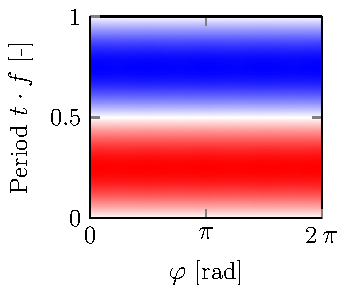
\includegraphics[]{/viscous_torque_0.pdf}
    % % \label{fig:TO-QPDx}
  % \end{subfigure}
  % \hfill
  % \begin{subfigure}[b]{0.3\textwidth}
    % \centering
    % \caption{$\zeta = \sfrac{\pi}{4}\,\si{\radian}$}
    % % \tikzsetnextfilename{viscous_torque_1}

\pgfplotsset{%
    colormap={bwr}{
      color=(blue);
      color=(white);
      color=(red);
    }%
}

\begin{tikzpicture}
  \begin{axis}[view={0}{90},
      xlabel={ $\varphi$ [rad] },
      xtick={0,3.1415,6.28},
      xticklabels={0,$\pi$,$2\,\pi$},
      height=50mm,
      width=55mm,
      % colorbar,
      % colorbar horizontal,
      % colorbar style={
        % title={\footnotesize Acoustic pressure $p_{\MR{a}}$},
        % at={(0,1.4)},
        % anchor=north west,
        % xticklabels={,,},
        % % xtick={0,0.5,1},
      % }
    ]
      \addplot3[surf,mesh/rows=50,shader=interp] table[x=phi,y=t,z=zeta1] 
      {\relPath/10_Figures/TikZ/Viscous_Torque.dat};

  \end{axis}
\end{tikzpicture}

    % 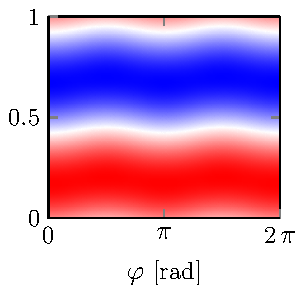
\includegraphics[]{/viscous_torque_1.pdf}
    % % \label{fig:TO-QPDkky}
  % \end{subfigure}
  % \hfill
  % \begin{subfigure}[b]{0.3\textwidth}
    % \centering
    % \caption{$\zeta = \sfrac{\pi}{2}\,\si{\radian}$}
    % % \tikzsetnextfilename{viscous_torque_2}

\pgfplotsset{%
    colormap={bwr}{
      color=(blue);
      color=(white);
      color=(red);
    }%
}

\begin{tikzpicture}
  \begin{axis}[view={0}{90},
      xlabel={ $\varphi$ [rad] },
      xtick={0,3.1415,6.28},
      xticklabels={0,$\pi$,$2\,\pi$},
      height=50mm,
      width=55mm,
      % colorbar,
      % colorbar horizontal,
      % colorbar style={
        % title={\footnotesize Acoustic pressure $p_{\MR{a}}$},
        % at={(0,1.4)},
        % anchor=north west,
        % xticklabels={,,},
        % % xtick={0,0.5,1},
      % }
    ]
      \addplot3[surf,mesh/rows=50,shader=interp] table[x=phi,y=t,z=zeta2] 
      {\relPath/10_Figures/TikZ/Viscous_Torque.dat};

  \end{axis}
\end{tikzpicture}

    % 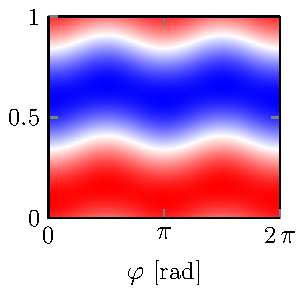
\includegraphics[]{/viscous_torque_2.pdf}
    % % \label{fig:TO-QPDt}
  % \end{subfigure}
  % \caption{Acoustic pressure $p_{\MR{a}}$ around spherical particle 
      % circumference ($\varphi$) in a two dimensional pressure wave field with 
      % three different phase shifts $\zeta$ plotted over one excitation period. 
      % The pressure amplitude is depicted qualitatively; red equals positive 
  % pressure and blue negative.}
  % \label{fig:TA-VT}
 % \end{figure}

Not only non-spherical objects can rotate due to the acoustics, but also 
spherical particles can rotate in an orthogonal two dimensional pressure wave 
field if two conditions are met: 1) the viscous losses inside the VBL $\delta$ 
around the particle are high enough; 2) the excitation of the two pressure 
waves is phase shifted.

If the two conditions are met, then the by $\zeta$ phase shifted excitation 
will lead to a local time-averaged streaming in the VBL of the particle that 
initiates the rotation. The final rotational velocity is when the particle 
accelerating torque form the local streaming flow equals the opposite directed 
Stokes' rotational drag torque~\cite{Lamprecht2017}. This rotational velocity 
is -- amongst other parameters -- proportional to the phase shift $\zeta$. 
Therefore, $\zeta + \sfrac{\pi}{2}$ will cause rotations opposite to a phase 
shift of $\zeta$. For neighboring superimposed pressure nodes along $\ex$ or 
$\ey$ the rotational direction is also opposite. We will discuss this kind of 
particle rotation more extensively in \cref{ch:viscoustorque}.

% \section{Python module for Acoustofluidic\label{sec:TA-python}}
